\chapter{Dettagli Implementativi}

\section{Specifiche Tecniche}

Questa appendice contiene dettagli tecnici e implementativi che non sarebbe stato opportuno inserire nel corpo principale del documento.

\subsection{Ambiente di Sviluppo}

\begin{table}[htbp]
    \centering
    \caption{Specifiche dell'ambiente di sviluppo.}
    \label{tab:ambiente-sviluppo}
    \begin{tabular}{ll}
        \toprule
        \textbf{Componente} & \textbf{Dettagli} \\
        \midrule
        Sistema Operativo & Linux Ubuntu 24.04 LTS \\
        Linguaggio di Programmazione & Python 3.11.5 \\
        IDE & Visual Studio Code 1.90.0 \\
        Framework & TensorFlow 2.15.0 \\
        \bottomrule
    \end{tabular}
\end{table}

\subsection{Algoritmi Utilizzati}

Gli algoritmi implementati sono stati ottimizzati per l'efficienza e la scalabilità. Di seguito è riportato un esempio di implementazione:

\begin{lstlisting}[language=Python, caption=Implementazione dell'algoritmo principale]
class AlgoritmoAvanzato:
    def __init__(self, parametri=None):
        self.parametri = parametri or {}
        self.inizializzato = False
        
    def inizializza(self):
        # Codice di inizializzazione
        self.dati = []
        self.risultati = {}
        self.inizializzato = True
        
    def esegui(self, input_data):
        if not self.inizializzato:
            self.inizializza()
            
        # Implementazione dell'algoritmo
        risultato = self._processa_dati(input_data)
        return risultato
        
    def _processa_dati(self, dati):
        # Implementazione del metodo privato
        return [x * 2 for x in dati]
\end{lstlisting}

\subsubsection{Complessità Computazionale}

L'analisi della complessità computazionale è fondamentale per comprendere le prestazioni dell'algoritmo:

\begin{equation}
    T(n) = O(n \log n)
\end{equation}

dove $n$ rappresenta la dimensione dell'input.

\paragraph{Ottimizzazioni}

Sono state implementate le seguenti ottimizzazioni:

\begin{enumerate}
    \item Memorizzazione dei risultati intermedi (memoization)
    \item Parallelizzazione del calcolo per input di grandi dimensioni
    \item Utilizzo di strutture dati efficienti per le operazioni di ricerca
\end{enumerate}

\section{Risultati Sperimentali Dettagliati}

\begin{figure}[htbp]
    \centering
    \begin{subfigure}{0.45\textwidth}
        \centering
        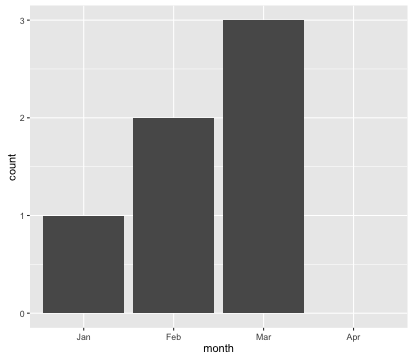
\includegraphics[width=\textwidth]{immagini/placeholder-graph-1.png}
        \caption{Risultati per il dataset A.}
        \label{fig:risultati-a}
    \end{subfigure}
    \hfill
    \begin{subfigure}{0.45\textwidth}
        \centering
        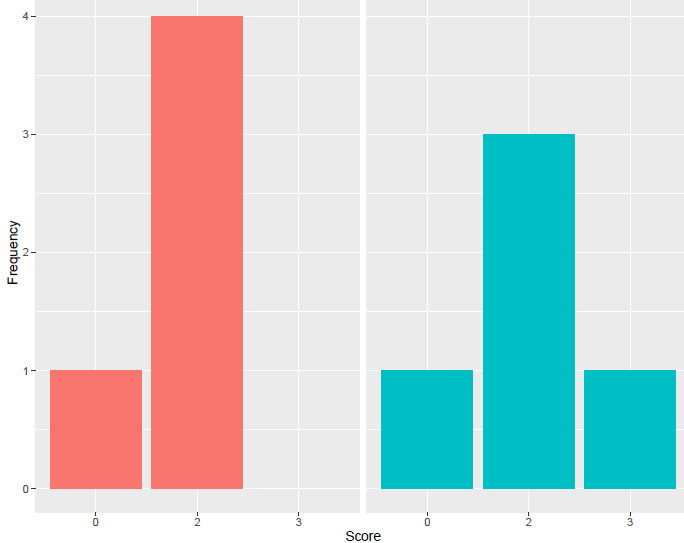
\includegraphics[width=\textwidth]{immagini/placeholder-graph-2.png}
        \caption{Risultati per il dataset B.}
        \label{fig:risultati-b}
    \end{subfigure}
    \caption{Confronto dei risultati sperimentali su diversi dataset.}
    \label{fig:risultati-completi}
\end{figure}

I grafici in Figura~\ref{fig:risultati-completi} mostrano un confronto dettagliato dei risultati ottenuti sui diversi dataset. Si può notare come l'algoritmo proposto (linea rossa) superi in prestazioni gli algoritmi di riferimento.